% !TeX spellcheck = es_ES
\documentclass[american,stu,biblatex,12pt,a4paper]{apa7}
\usepackage[autostyle,thresholdtype=words]{csquotes}
\usepackage[T1]{fontenc}
\usepackage[utf8]{inputenc}
\usepackage[spanish]{babel}
\usepackage{graphicx}
\usepackage{xparse}
\usepackage{amsmath,amsfonts,amssymb,relsize}
\usepackage{tabularx}
\usepackage{geometry}
\usepackage{listings}
\geometry{ a4paper, total={170mm,257mm}, left=20mm, top=20mm,}

\usepackage[style=apa, backend=biber]{biblatex}
\addbibresource{references.bib}




%%Cover page
\makeatletter
\long\def\campus#1{\long\def\@campus{#1}}

\renewcommand{\maketitle}{	
	\check@author
	\begin{titlepage}
		\centering
		
\includegraphics[scale=0.3]{imagenes/tec.png}\\
		\vfill
		{\large \displayaffiliations\par}
		\vfill
		{\large \@title \par}
		{\@shorttitle  \par}
		\vfill
		{\scshape\large Estudiantes: \par}
		{\large \displayauthors \par}
		\vfill
		{\large \scshape Sede \@campus \par}
		{\large \@duedate \par}
	\end{titlepage}
	\newpage
}
\makeatother


\newcommand{\paraphrase}[3]{
	\textcite{#1}#3 (#2)
}

\makeatletter
\renewenvironment*{blockquote}{%
	\setlength{\leftmargini}{1in}\csq@getcargs{\csq@bquote{}{}}
}
\makeatother
\SetCiteCommand{\textcite}
\SetBlockThreshold{39}

\setlength{\parindent}{0.5in}
\renewcommand{\baselinestretch}{2} %%interlineado


\newcommand{\myItem}[1]{\item #1}
\newcommand{\myRow}[1]{#1\\\hline}

\NewDocumentCommand \myItemize{ > { \SplitList { ? } } m }{
	\begin{itemize}
		\ProcessList{#1}{\myItem}
	\end{itemize}
}

\NewDocumentCommand \myEnumerate{ > { \SplitList { ? } } m }{
	\begin{enumerate}
		\ProcessList{#1}{\myItem}
	\end{enumerate}
}

\newcommand{\subsectionInList}[1]{
\addcontentsline{toc}{subsection}{#1} \textbf{#1}
}

\NewDocumentCommand{\resultados}{ > { \SplitList { ? } } m }{
\begin{center}
	\begin{tabularx}{\textwidth}{|X|c|X|}
		\hline
		Requerimiento&Estado&Observaciones\\\hline
		\ProcessList{#1}{\myRow}
	\end{tabularx}
\end{center}
}


\begin{document}
	\authorsaffiliations{
	Instituto Tecnológico de Costa Rica\\
	Unidad de Computación
	}
	\course{Sistemas de información geográfica
	}
	\title{Segundo proyecto programado\\{\normalsize Documentación externa}}
	\shorttitle{}
	\authorsnames{José Daniel Villegas Paniagua}
	\campus{San Carlos}
	\duedate{18 de noviembre del 2021}
	\maketitle
	
	\renewcommand{\contentsname}{\raggedright\LARGEÍndice}
	\tableofcontents
	\newpage
	%\renewcommand{\section}{\@startsection {section}{1}{\z@}
	{\b@level@one@skip}{\e@level@one@skip}
	{\normalfont\Large\bfseries}
}

\renewcommand{\subsection}{\@startsection {subsection}{2}{\z@}
	{\b@level@two@skip}{\e@level@two@skip}
	{\normalfont\large\bfseries}
}

\renewcommand{\subsubsection}{\@startsection {subsubsection}{3}{\z@}
	{\b@level@three@skip}{\e@level@three@skip}
	{\normalfont\normalsize\bfseries}
}
	
	
	% !TeX spellcheck = es_ES
\section{Introducción}
Los usuarios de servicios de buses del país no siempre cuentan con las mejores herramientas o productos que les indiquen cuales son las mejores opciones de viaje por lo que se suelen optar simplemente por la que recuerdan o la que se sabe "del boca a boca" por lo que brindar una información más precisa de mano de la ARESEP y otros geoservicios como lo puede ser OpenStreetMaps puede implicar una mejora significativa en la forma en que se percibe viajar en bus.

Esto ya abre a más posibilidades a servicios más complejos como cuáles paradas debe visitar el usuario o debería visitar para hacer su viaje el más optimo y no pasar tanto tiempo viajando y más tiempo en su destino de preferencia.
\newpage 

	
	% !TeX spellcheck = es_ES
%analizar los puntos a tratar en la evaluación, considerando estos como
%requerimientos de un proyecto de software o como las preguntas o situaciones a resolver
%en un proceso de indagatoria (investigación).

%metodologías o medios necesarios para brindar una posible solución o abordaje al problema.

%diagramas de conceptos, técnicas, herramientas, o ejemplos prácticos de situaciones en donde se visualice la problemática o situación
%planteada, evitando a toda costa la utilización de descripciones o prosa confusa y poco
%relevante sobre el punto a tratar.

\section{Análisis del problema}
\subsection{Herramientas}

Para las rutas de buses se usarán los geoservicios que brinda aresep, esto según como lo indica el requerimiento del proyecto para luego ser cargados a la base de datos, por lo que se debe buscar una herramienta que permita facilitar el proceso, de igual forma con la calles de alguna ciudad de Costa Rica, en este caso con OpenStreetMap.

En cuanto a la visualización e interacción de la información a nivel del cliente, se planea utilizar leaflet y svelte como framework con nodejs y expressjs al lado del backend debido a su portabilidad y facilidad para configurar para poder tenerlo en ejecución.

\subsection{Limitaciones técnicas}
Para entrar en materia se debe comprender las limitaciones del servidor donde se encuentra alojada la base de datos solamente tiene 4Gb de ram por lo que no se puede pensar en tener más de una ciudad en calles para hacer el análisis (puesto que podría llegar a superar las diez mil calles); debido a que la comparación de intersección o cercanía entre geometrías es una operación de N calles por M rutas.

Por lo anteriormente mencionado se debe también en recortar tiempo o procesamientos, para esto se puede usar un cursor para las calles y cada que encuentra una ruta cerca deje de realizar las comparaciones, por ejemplo:

\begin{lstlisting}
	FOR calle IN calles LOOP
		Insert into tabla_intermedia
		SELECT calle.id FROM aresep ar
			WHERE ST_DWITHIN(ar.geom,calle.geom,distancia)
			LIMIT 1;
	END LOOP;
\end{lstlisting}

El problema con lo anterior es que no estaría usando el indice y no existiría una relación calle-ruta, por lo que otra alternativa sería aplicar el cursor a la tabla del aresep (filtrado) y que a pesar de que usa el indice y se podría hacer fácilmente la relación $calle\longleftrightarrow ruta\longleftrightarrow parada$, se estaría ejecutando el análisis sobre todas las rutas y calles (ya filtradas); ejemplo de código:

\begin{lstlisting}
	FOR rutas IN rutas_filtradas LOOP
	Insert into tabla_intermedia
	SELECT id,ruta.id FROM calles
		WHERE filtado_en_calle
			AND ST_DWITHIN(ar.geom,calle.geom,distancia);
	END LOOP;
\end{lstlisting}

\hfill

Con el código anterior se permitiría tener la siguiente estructura:

\begin{center}
	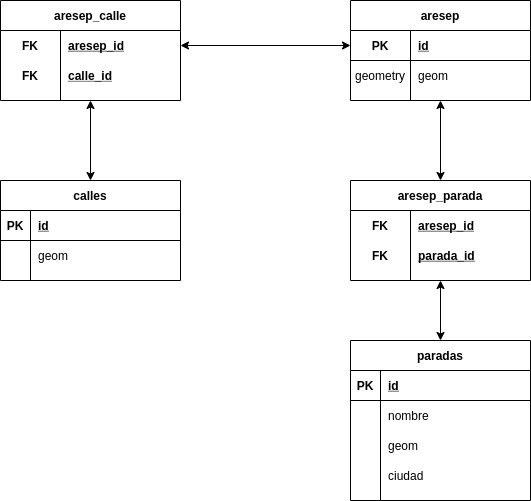
\includegraphics[scale=.65]{imagenes/diagram_db.png}
\end{center}

\break
\subsection{Colisión e indices}

Para determinar de forma más rápida se debe pensar en una forma que permita hacer una análisis rápido y de bajo costo que permita descartar las calles que no pasan por las rutas del ARESEP, por ejemplo un bounding box que encasille las rutas y para luego con solo una geometría descartar las rutas (lineas negras).

\begin{center}
	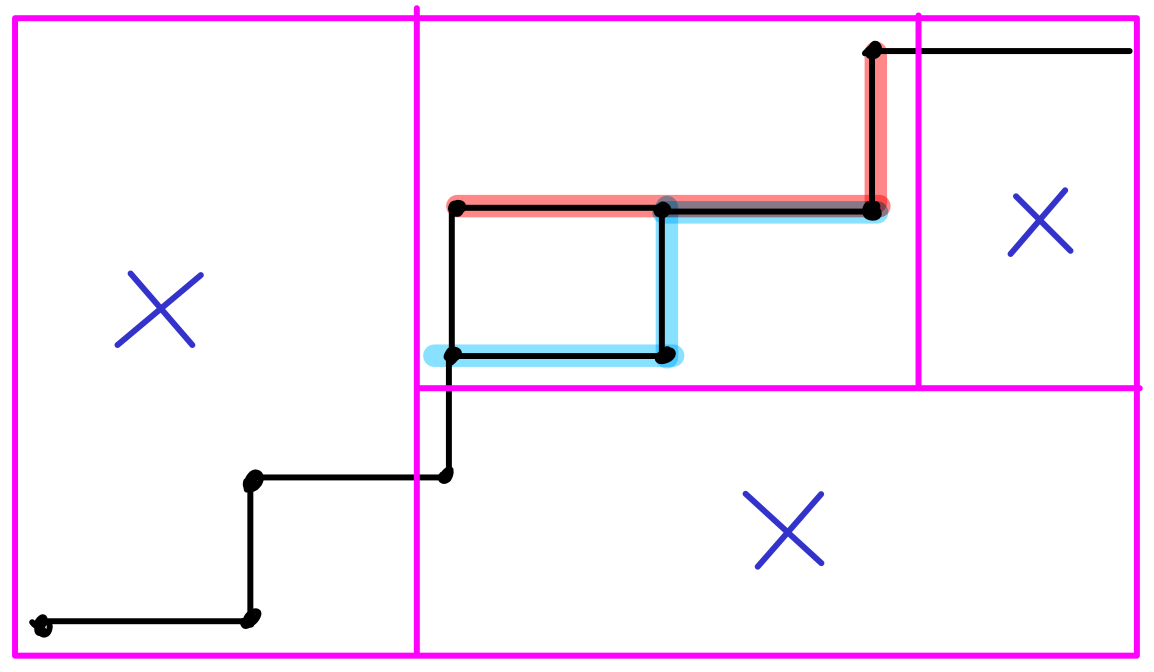
\includegraphics[scale=.4]{imagenes/colisiones.png}	
\end{center}

\subsection{Creación de la topología}
En cuanto a la creación de la topología se debe plantear la creación de los vértices solamente por las calles por las cuales pasan las rutas:

\begin{lstlisting}
	SELECT pgr_createTopology('tabla',dist,'geom','id',
	rows_where:='(SELECT true from aresep_calle ac
				where ac.calle_id=id)',
	clean:=true);
\end{lstlisting}

\subsection{Ruta más corta}
Para la ruta más corta hay 2 opciones:
\myEnumerate{
	Marcar inicio y destino y luego marcar las paradas por donde se pasa.?
	Recopilar todas las paradas por donde pasan las rutas del ARESEP y en base a esto ejecutar múltiples dijkstras del inicio al punto b,c,d hasta el destino.
}

Ejemplo del punto 2:


\begin{center}
	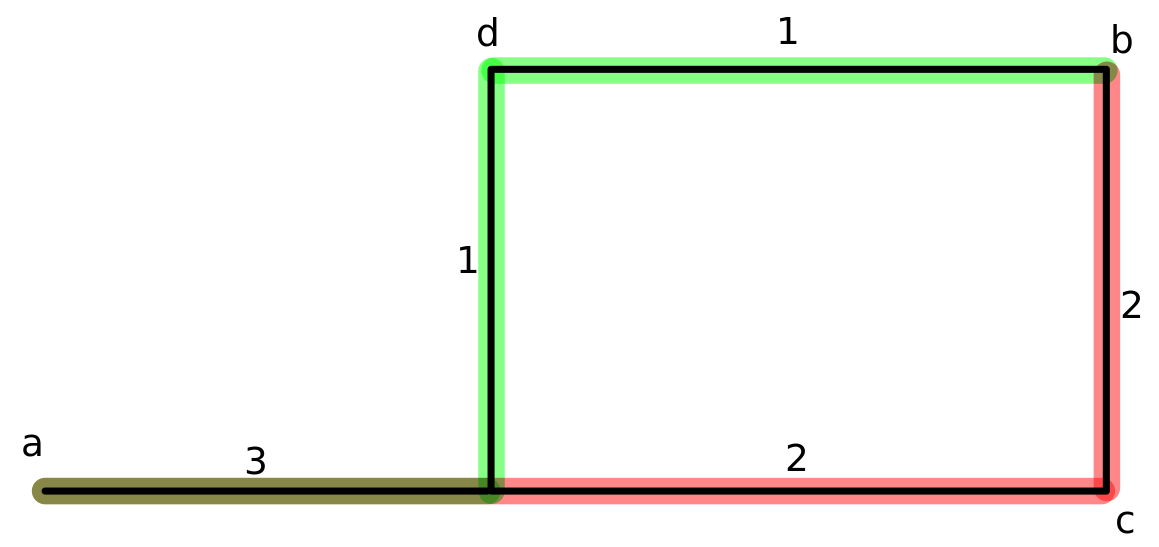
\includegraphics[scale=.4]{imagenes/dijkstra.png}	
\end{center}

La ruta más corta de $a\rightarrow b$ es $a\rightarrow d\rightarrow b$ (linea verde), pero la ruta del ARESEP (rojo) de $a\rightarrow b$ no pasa por d; por lo que en este caso sería un dijkstra de $a \rightarrow c$ y luego de $c\rightarrow b$.

\newpage

	
	% !TeX spellcheck = es_ES
\section{Solución del problema}


%https://gis.stackexchange.com/questions/374091/when-to-use-gist-and-when-to-use-sp-gist-index
%https://blog.crunchydata.com/blog/the-many-spatial-indexes-of-postgis
En cuanto a los \textbf{indices} en las tablas se tienen a GIST y SPGIST; según el usuario \textbf{geozelot} menciona que SPGIST necesita menos espacio que que GIST por lo que es algo a considerar además \textbf{PAUL RAMSEY} menciona  que SPGIST supera a GIST cuando se procesan datos que no se superponen sobre otros (caso de las calles), por lo que para las calles se estaría utilizando SPGIST y para las rutas del ARESEP que suelen pasar varias por el mismo punto, se estaría utilizando GIST.

\newpage

	
	% !TeX spellcheck = es_ES
\section{Análisis de resultados}

\vspace{10mm}

\resultados{
	Implementación del visor&Completo&?
	Diseño de base de datos&Completo&?
	Registro de datos (lineas de bus, vías, y paradas)&Completo&?
	Carga de capas en el visor&Incompleto&Solo carga las paradas de buses?
	Ruteo punto de origen y destino y despliegue de resultados geográficos&&?
	Despliegue de detalles en la ruta resultante&&?
	Documentación interna&Completo&?
	Documentación Externa&Completo&
}

\newpage

	
	% !TeX spellcheck = es_ES
\section{Conclusiones}
\newpage 

	
	% !TeX spellcheck = es_ES
\section{Recomendaciones}
\newpage 

	
	\newpage
	\nocite{*}
	\addcontentsline{toc}{section}{Referencias}
	\printbibliography
	
	\newpage
	\section{Anexos}
	\subsection{Enlace a video de youtube}
	\url{https://youtu.be/H61JqlYFue4}
	\subsection{Enlace a repositorio en github}
	\url{https://github.com/jdv98/sig_proyecto2}
	
\end{document}